\documentclass[10pt, journal]{IEEEtran}			% draftcls, http://vesta.informatik.rwth-aachen.de/ftp/pub/mirror/ctan/macros/latex/contrib/IEEEtran/IEEEtran_HOWTO.pdf
\setlength{\parindent}{0em} 					% Absatzeinrücken verhindern
\usepackage[utf8]{inputenc}
\usepackage[ngerman]{babel}
\usepackage[T1]{fontenc}
%\usepackage{cmbright}							% Schriftart https://tug.org/FontCatalogue/
\usepackage{amsmath, amsthm, amssymb}
\usepackage{mathtools}
\setlength\abovedisplayshortskip{-5pt}  		% Kopfabstand von Formeln	
\setlength\abovedisplayskip{+7pt} 	
\setlength\belowdisplayskip{+7pt} 	
\usepackage{siunitx}							% Si Einheiten
\usepackage{graphicx}
\usepackage{multirow}  							% Multirow in Tabellen
\usepackage{arydshln}  							% Punkt/strich Linen in Tabellen
\usepackage{pdflscape} 							% Seite kann mit landscape in Querformat dargestellt werde
\usepackage{caption}
\usepackage{here}
\usepackage{graphicx}  							% Tab neben Bilder
\usepackage{booktabs}  							% Tab neben Bilder
\usepackage{cite}								% IEEE Zitate


\begin{document}
	\title{Variable Stromsenke\\Messtechnik 2, Fachartikel}
	\author{Johannes Rothe} 
	\markboth{Fachartikel Variable Stromsenke}{Rothe}
	\maketitle 

	\input{section/Einführung}
	
	\section{Schaltung}
\label{sec:Schaltung}

\begin{figure}[!h]
	\centering
	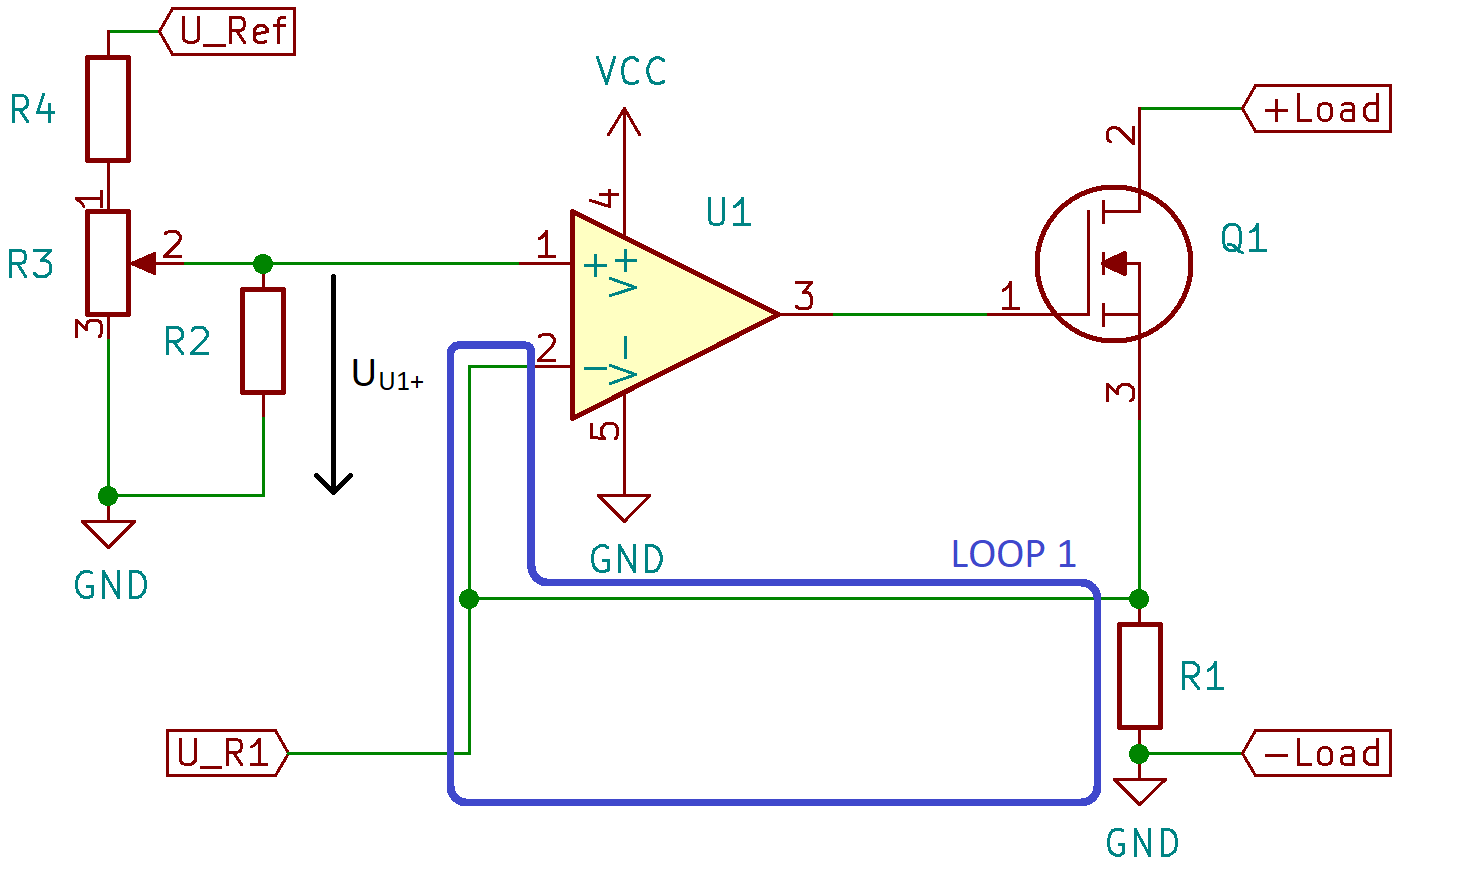
\includegraphics[width=0.5\textwidth]{Bilder/G_Schaltung.PNG}
	\renewcommand*\figurename{Schaltung}
	\caption{Grundschaltung}
	\label{sch:Grundschaltung}
\end{figure}

Die Grundlage dieser Schaltung geht auf die Shuntmessung und deren grundlegenden Zusammenhang von $U_{R1} = I_{R1} \cdot R1$ zurück.
Der N-Kanal MOSFET $Q_{1}$ wird bei dieser Schaltung im Widerstandsbereich betrieben und ist somit die einstellbare Last. 
Die elektrische Energie wird dort in Wärme umgewandelt.
Der Operationsverstärker (kurz OP) steuert sein Ausgangssignal so, dass am invertierenden (-) und nicht-invertierenden Eingang (+), 
keine Spannungsdifferenz herrscht.
Mit anderen Worten: Die Spannung über $R1$ ist gleich der Referenzspannung $U_{U1+}$ 
(einstellbarer Spannungsteiler mit $R2$, $R3$ und $R4$).
Somit ergibt sich der Zusammenhang von $I_{R1}$ und $U_{U1+}$ wie folgt:

\begin{equation}
	I_{R1} = \frac{U_{U1+}}{R1}
	\label{eq:IR1}
\end{equation}

In dem Spannungsteiler, der Referenz, ist bereits auf einen möglichen Fehlerfall und deren Folgen eingegangen.
Der Widerstand $R2$ verhindert, dass bei einem Kontaktproblem am Potentiometer die Spannung $U_{U1+}$ nicht undefiniert bleibt 
sondern auf GND Potential gelegt wird. 
Somit ist sichergestellt, dass die Last im Fehlerfall hochohmig geschaltet wird. 
Die Formel \ref{eq:UOp+} zu diesem Spannungsteiler beschreibt die Spannung am Eingang $U1+$. Unter anderem in Abhängigkeit des Winkels 
und des maximalen Winkels von dem Potentiometer $R3$.
Dabei ist $\alpha$ der Winkel zwischen Schleifer (Kontakt 2) und Kontakt 3.
Diese Formel kann für beide Anschläge zu den Formeln \ref{eq:UU1max_min} stark vereinfacht werden.
Die allgemeine Formel des Spannungsteilers lässt einen nahezu linearen Zusammenhang zwischen Spannung $U_{U1+}$ 
und Winkel $\alpha$ erkennen. Zur Berechnung des maximalen Stromes $I_{R1,max}$ genügt die Betrachtung der Spannung 
$U_{U1+,max}$ (Formel \ref{eq:UU1max_min}).

\begin{equation}
	U_{U1+} = U_{Ref} \cdot \frac{\frac{R2 \cdot R3 \cdot \frac{\alpha}{\alpha_{max}}}
									{R2 + \big(R3 \cdot \frac{\alpha}{\alpha_{max}}\big)}}
							{R4 + \frac{R2 \cdot R3 \cdot \frac{\alpha}{\alpha_{max}}}	
									{R2 + \big(R3 \cdot \frac{\alpha}{\alpha_{max}}\big)} + \Big(R3 \cdot 
									\frac{(\alpha_{max} - \alpha)}{\alpha_{max}} \Big)}
	\label{eq:UOp+}
\end{equation}
\vspace{0,1cm}
\begin{equation}
	U_{U1+,max} = U_{Ref} \cdot \frac{\frac{R2 \cdot R3}{R2 + R3}}
							{R4 + \frac{R2 \cdot R3}{R2 + R3}}
		\qquad		
	U_{U1+,min} = 0
	\label{eq:UU1max_min}
\end{equation}

\begin{figure}[!h]
	\centering
	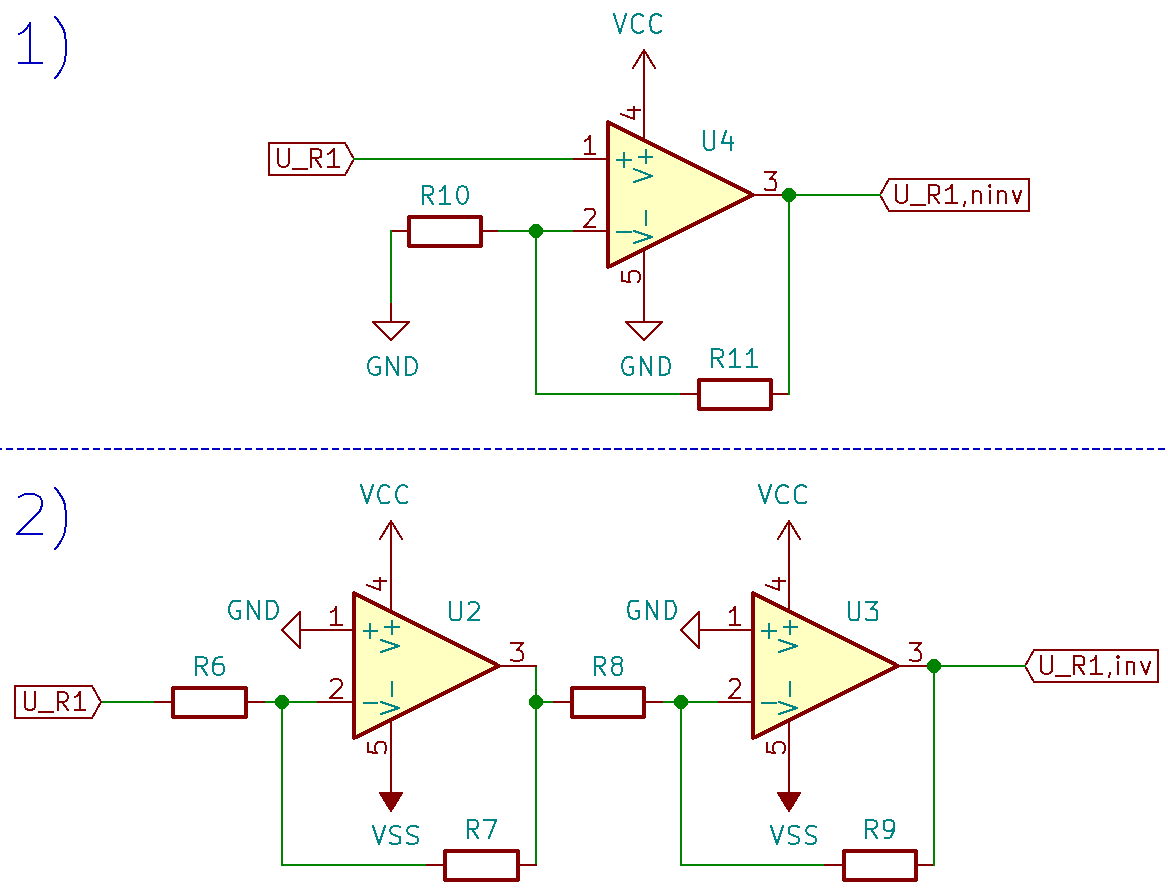
\includegraphics[width=0.45\textwidth]{Bilder/OP_Schaltung_analyse.PNG}
	\renewcommand*\figurename{Schaltung}
	\caption{Operationsverstärkerschaltungen zur Aufbereitung des Shuntsignals $U_{R1}$\\
		1) nicht-invertierender Verstärker\\
		2) zwei invertierende Verstärker }
	\label{sch:OP_Verstärkung}
\end{figure}

Damit der fließende Strom, mit beispielsweise einem Mikrocontroller, bestimmt werden kann, muss die Spannung $U_{R1}$ verstärkt werden. 
Dazu eignen sich zwei einfache Schaltungen.

Um kleine Spannungen mit Faktor größer 1,5 zu verstärken eignet sich die erste Schaltung. 
Die Schaltung des nicht-invertierenden Verstärkers (Schaltung. \ref{sch:OP_Verstärkung}.1) eignet sich daher für große Strombereiche bei 
relativ großem Shunt-Widerstand $R1$. 
Die Verstärkung ($V_{U4}$) berechnet sich nach:

\begin{equation}
	V_{U4} = 1+ \frac{R11}{R10}
	\label{eq:V_nichtInv}
\end{equation}

Zu erkennen ist, dass dieser Verstärker mathematisch keine $V$ $\leq 1$ realisiert werden kann.


In Schaltung Nr.2 sind zwei invertierende Verstärker hintereinander geschaltet. 
Diese ist für Strombereiche mit sehr großem Shunt-Widerstand $R1$ geeignet, da eine Verstärkung kleiner 1 
realisiert werden kann.
Die Verstärkung ($V_{ges}$) berechnet sich nach:

\begin{equation}
	V_{U2} = - \frac{R7}{R6}  
		\qquad
	V_{U3} = - \frac{R9}{R8}
	%\label{eq:V_Inv}
\end{equation}
\vspace{0cm}
\begin{equation}
	V_{ges} = V_{U2} \cdot V_{U3}
	\label{eq:V_Inv}
\end{equation}

Diese ist mit mehr Schaltungsaufwand verbunden, da aufgrund der Invertierung des Signals eine 
Bipolare-Spannungsversorgung nötig ist. 


	
	\section{Schaltung Auslegen}

Falls Sie die Schaltung zusammenbauen möchten sollte der nachfolgende Teil einmal vollständig gelesen werden.
Sie legen Ihre Präferenzen fest, berechnen die Werte und suchen dann passende Bauteile heraus.
\newline

Wenn der MOSFET ($Q1$) im Betrieb hochohmig geschaltet werden soll, wird für die Regelung ($U1$), 
ein sogenannter Rail to Rail Operationsverstärker benötigt. 
Diese Art von OP`s, können ihre Ausgangsspannung bis nah an die Versorgungsspannung heran durchschalten.

Bei der Versorgung des OP`s muss darauf geachtet werden, dass das mögliche Ausgangspotential größer ist als $U_{GS(th),max}$.
$U_{GS(th),max}$ ist die maximale Gate-Source Schwellspannung (Englisch: Gate-Source Threshold Voltage) des MOSFET. 
Beim unterschreiten dieser, kann der MOSFET nicht vollständig durchschalten.
Bei einer Versorgungsspannung von \SI{5}{\volt} empfehlen sich sogenannte Logic-Level MOSFET`s 
(IRL(\textit{X}) \cite{LL_MOSFET}).

Neben diesem Wert sollte ebenfalls auf $U_{DS}$ (Drain-Source Durchbruch Spannung) geachtet werden. Diese bestimmt die 
spätere maximale Spannung der Last ($U_{L,max}$)\footnote{In Abb.\ref{sch:Grundschaltung} Spannung zwischen +Load und -Load}. 
Lesende, die mit dem Kirchhoffschen-Maschengesetz vertraut sind werden sagen, dass das noch nicht ganz stimmt.
Die Masche für die maximale Spannung ist:
\begin{equation}
	U_{L,max} = (I_{L} \cdot R1) + U_{DS}
	\label{eq:U_Lmax}
\end{equation}

Wenn bei dem Einschalten von einem Laststrom $I_{L} = \SI{0}{\ampere}$ ausgegangen wird, wird der erste Term aus Formel \ref {eq:U_Lmax} 
$= 0$ und $U_{L,max}$ ist somit gleich $U_{DS}$. 


Kleine Anmerkung: Wer ein bisschen bastelt, hat bestimmt ein IRFP450 \cite{IRFP450} herumliegen. 
Der eignet sich sehr gut: $U_{GS(th),max} = \SI{4}{\volt}$, $U_{DS} = \SI{500}{\volt}$, $I_{D} = \SI{14}{\ampere}$ 
und $R_{DS(on)} = \SI{0,4}{\ohm}$ (Bedingung Beachten \cite{IRFP450}).

Der Shunt-Widerstand $R1$ sollte allgemein nicht zu klein ausfallen.
Bei kleiner Loop (1)- und Referenzspannung, können elektromagnetische Störungen von Außen überwiegen.

Die minimale ohmsche Last die simuliert werden kann, ist:
\begin{equation}
	R_{L,min} = R1 + R_{DS(on)}
	\label{eq:R_Lmin}
\end{equation}

%\begin{equation}
%	P_{R1,max} = I_{L,max}^2  \cdot R1
%	\label{eq:P_R1max}
%\end{equation} 

\subsection{Beispiel} 
\label{sec:Bsp}
Nehmen wir ein IRFP450 \cite{IRFP450}, $R1 = \SI{100}{m\ohm}$ und $U_{U1} = U_{Ref}= \SI{12}{\volt}$.
Wir legen $I_{L´,max} = \SI{7}{\ampere}$, $U_{L,max} = \SI{20}{\volt}$ und $U1$ als Rail to Rail Operationsverstärker fest.

Somit ergeben sich für $P_{R1,max}$ und $U_{U1+,max}$: 
\begin{equation}
	P_{R1,max} = I_{L,max}^2  \cdot R1 = (\SI{7}{\ampere})^2 \cdot \SI{0,1}{\ohm} = \SI{4,9}{\watt}
\end{equation}
\begin{multline}
	\begin{split}
		U_{U1+,max} &= I_{L´,max} \cdot R1 = \SI{7}{\ampere} \cdot \SI{0,1}{\ohm} = \SI{0,7}{\volt} \\
		&= U_{R1,max}
	\end{split} 
\end{multline}


Bei der Referenz legen wir $R3 = \SI{10}{k\ohm}$ und $R2 = \SI{100}{k\ohm}$ fest. Formel \ref{eq:UOp+} 
%($R23$ siehe Formel \ref{eq:R23}) 
wird nach $R4$ umgestellt:
\begin{multline}
	\begin{split}
		R4 &= \biggl( \frac{U_{Ref} \cdot \frac{R2 \cdot R3}{R2 + R3}}{U_{U1+,max}}\biggr) - \frac{R2 \cdot R3}{R2 + R3}\\
		&= \biggl( \frac{\SI{12}{\volt} \cdot \SI{9,09}{k\ohm}}{\SI{0,7}{\volt}}\biggr) - \SI{9,09}{k\ohm} = \SI{146,73}{k\ohm}
	\end{split}
\end{multline}

Einen Widerstand mit $R = \SI{146,73}{k\ohm}$ wird es wahrscheinlich nirgends zu kaufen geben. 
Nach der E 96-Reihe (Nach DIN 41426 \cite{E-Reihen}), ist der nächste nähere Wert $147 k\Omega$. 
Durch diesen anderen Wert ergibt sich $I_{L,max} = \SI{6,988}{\ampere}$.


\subsection{EMV-Aspekte} 
\label{sec:EMV}
Eine Leiterschleife, senkrecht von einem magnetischen zeitlich-veränderlichen Fluss durchströmt, induziert eine elektrische 
Spannung. 
Die induzierte elektrische Spannung ist von der Fläche und der  magnetischen Flussdichte abhängig. Um diesen Störeinfluss 
%(wie im Abschnitt \ref{sec:Schaltung} angesprochen) 
zu minimieren, sollte der Loop 1 (Abb. \ref{sch:Grundschaltung}) möglichst kurz und eine kleine Innenfläche vorweisen. 
Bei Anwendung in Bereichen mit großen Störeinflüssen sollte der Loop 1 zusätzlich geschirmt 
werden (Bsp: Innenleiterbahn oder $\mu$-Metall). 
%Um Störeinflüsse an der Referenz zu minimieren sollte ein Kondensator parallel zu $R2$ möglichst nah am  Operationsverstärker 
%eingebracht werden.
Weniger kritisch ist die Referenz am Eingang $U1_{+}$. 
Hier sollte dennoch ein Kondensator parallel zu $R2$, möglichst nah am Operationsverstärker, 
eingebracht und lange Leiterbahnen/Zuleitungen vermieden werden.

\subsection{Temperaturabhängigkeit/-eigenschaft}

Die Temperatureigenschaften von dem MOSFET $Q1$ werden nicht beachtet, da dieser gesteuert wird. Die Temperaturabhängigkeit ist 
wesentlich von der Referenzspannung $U_{U1+}$ und dem Shunt $R1$ abhängig. Um den maximalen Fehler zu berechnen ist der TCR-Wert 
(Temperature Coefficient of Resistances), in [PPM/°C], wichtig. 
Dieser beschreibt die Widerstandsänderung aufgrund von Temperaturänderung. 
Für Widerstände gilt: (\cite{TCR_rechnen}, Seite 23)

\begin{equation}
	\label{eq:TCR}
	\Delta R_{max} = \Delta R + (T_{R,max} - \SI{25}{\celsius}) \cdot TCR_{R} \cdot10^{-4}
\end{equation}

\begin{table}[h!]
	\centering
	\caption{Beschreibung zur Formel \ref{eq:TCR}}
	\label{tab:Beschreibung_TCR}
	\normalsize
	\begin{tabular}{l|l}
		Term & Beschreibung \\
		\hline
		$\Delta R_{max}$& Resultierende maximale Toleranz[\%]\\
		$\Delta R$		& Widerstandstoleranz [\%] \\
		$T_{R,max}$		& Max. Temperatur am/im Widerstand [°C]\\
		$TCR_{R}$		& TCR-Wert des Widerstandes [PPM/°C]\\
	\end{tabular}
\end{table}

Um den Temperatureinfluss zu minimieren, sollten Widerstände konstant/nah bei \SI{25}{\celsius} betrieben werden. 
Der Shunt-Widerstand wird im Betrieb gegebenenfalls mit viel Leistung belastet. 
Hierbei sollte für ausreichend Kühlung gesorgt 
und bei der Fehlerrechnung der maximale Fehler nach Formel \ref{eq:TCR} beachtet werden.
Das Gehäuse des MOSFET sollte groß gewählt werden, damit die gegebenenfalls hohe anfallende 
Leistung, mit geringem thermischen Widerstand an den Kühlkörper abgegeben werden kann.
Die Kühlkörperberechnung/Auslegung ist nicht Teil dieses Artikels. 
Unter Bedingungen\footnote{$P_{L} \approx \SI{72}{\watt}$, \SI{30}{\second} Anzeit, \SI{10}{\minute} Auszeit} 
genügt ein relativ kleiner Kühlkörper von $\approx \SI{96,2}{c\meter^3}$.
Dabei wir die anfallende Wärme primär im Material gespeichert. 
Die Abgabe der gespeicherten Energie erfolgt größtenteils während der Auszeit.\\

Die restliche Schaltung ist thermisch und räumlich von diesen zwei zu kühlenden Bauteilen zu trennen.
Im Allgemeinen hat ein Schaltung eine höhere Genauigkeit, wenn diese bei konstanter und 
geringer Temperatur betrieben wird.
	
	\section{Simulation}

Die Grundlage der Simulation bildet die Grundschaltung und die Operationsverstärkerschaltung zur Aufbereitung des Shuntsignals $U_{R1}$ 
(Kapitel \ref{sec:Schaltung}). 
Die Schaltungen wurden in dem Simulationsprogramm LTspice\footnote{Wurde 1999 von Linear Technology einem 
US-Amerikanischen Halbleiter- und Softwarehersteller entwickelt.} aufgebaut. 
Zur Vereinfachung wurde $U_{U1+}$ mit einer Spannungsquelle simuliert und nicht mit der Schaltung $R2$ bis $R4$.
Die übrigen Widerstandswerte sind nach Tabelle \ref{tab:Werte_Fehler_Beispiel} festgelegt worden.
$Q1$ ist als ein IRFP240 \cite{IRFP250} simuliert.
Die Versorgungsspannungen und maximalen U/I-Werte der Last wurden nach Beispiel \ref{sec:Bsp} festgelegt.\\

\begin{table}[h!]
	\centering
	\caption{Beispiel Bauteile und Werte}
	\label{tab:Werte_Fehler_Beispiel}
	\normalsize
	\begin{tabular}{c|c|cc}
		Bauteil & Wert & Toleranz & $\Delta$ Wert\\
		\hline
		U2 bis U4 & LTC2057 & \cite{LTC2057} & --\\
		\multirow{2}{*}{R1}  & \multirow{2}{*}{\SI{100}{m\ohm}} & 0,5 \%,  & \multirow{2}{*}{0,762 m$\Omega$}\\
		&& TCR: 75 PPM/°C &\\
		R10 & $5 k\Omega$ & 1 \% & \SI{50}{\ohm} \\
		R11 & $15 k\Omega$ & 1 \%& \SI{150}{\ohm}\\
		R6  & $5 k\Omega$ & 1 \% & \SI{50}{\ohm} \\
		R7	& $5 k\Omega$ & 1 \% & \SI{50}{\ohm} \\
		R8  & $5 k\Omega$ & 1 \% & \SI{50}{\ohm} \\
		R9  & $20 k\Omega$ & 1 \%& \SI{200}{\ohm}\\
	\end{tabular}
\end{table}

\begin{figure}[!h]
	\centering
	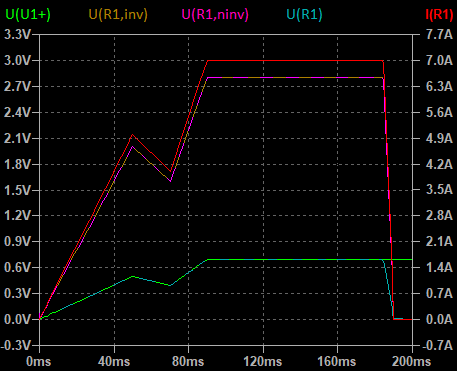
\includegraphics[width=0.45\textwidth]{Bilder/Simu_Kleinsignale.png}
	\renewcommand*\figurename{Diagramm}
	\caption{Simulation über 200ms für $U_{U1+}$, $U_{R1,inv}$, $U_{R1,ninv}$, $U_{R1}$ und $I_{R1}$}
	\label{simu:Kleinsignale}
\end{figure}

\begin{figure}[!h]
	\centering
	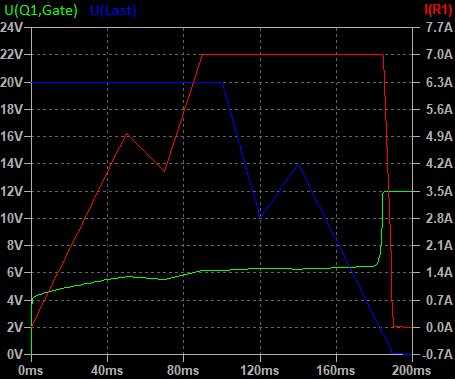
\includegraphics[width=0.45\textwidth]{Bilder/Simu_grossignale.png}
	\renewcommand*\figurename{Diagramm}
	\caption{Simulation über 200ms für $U_{Q1,Gate}$, $U_{Last}$ und $I_{R1}$}
	\label{simu:Großsignale}
\end{figure}


Im Diagramm \ref{simu:Kleinsignale} ist zu sehen, dass die Spannung $U_{U1+}$ bis \SI{90}{m\second} 
auf die festgelegten \SI{0,7}{\volt} eingestellt wird. Entsprechend folgt der gesteuerte Strom $I_{R1} = I_{Q1}$.
Die Spannung $U_{Q1,Gate}$ erhöht sich aufgrund der Gate-Source Schwellspannung nahezu sofort auf \SI{4}{\volt}.
Zu erkennen ist, dass bei einer Versorgungsspannung von \SI{5}{\volt} des Operationsverstärkers $U1$ der 
MOSFET $Q1$ für den gewünschten Strom von \SI{7}{\ampere} nicht genügend Gate-Source Spannung anlegen könnte.

Wenn ab $t \geq 100ms$ die Spannung an der Last linear sinkt, so ändert sich der Strom durch die Last nicht.
Ab einem $U_{Last} \lessapprox \SI{1,5}{\volt}$ ist der konstante Bereich erschöpft. 
An diesen Punkt kann der MOSFET $Q1$ keinen kleineren $R_{L}$ als $R_{L,min}$ (Formel \ref{eq:R_Lmin}) imitieren.
Für Spannungen $U_{Last} \lessapprox \SI{1,5}{\volt}$ gilt:

\begin{equation}
	I_{L} = \frac{U_{L}}{R_{L,min}}
\end{equation}

Ab einer Spannung $U_{Last} \lessapprox \SI{2}{\volt}$ steigt die Ausgangsspannung von $U1$ ($= U_{Q1,Gate}$) stark an, 
um $Q1$ niederohmiger zu schalten.
Diese Ausgangsspannung kann keinen Wert über \SI{12}{\volt} annehmen da dies das Maximum der Versorgung ist.

Die Schaltungen des invertierenden und nicht-invertierende Verstärkers verstärken beide, wie berechnet, 
die Shuntspannung $U_{R1}$ mit Faktor vier.



	
	\section{Grenzen und Fehler}
\label{sec:Grenzen}

\subsection{Grenzen}
Ein diskretes Halbleiterelement hat immer eine maximale Leistung (meist als $P_{tot}$ bezeichnet), die es umsetzten kann.
Im Fall unseres beliebten IRFP450 sind dies $P_{tot} = \SI{190}{\watt}$ 
\footnote{Im Datenblatt des IRFP450 \cite{IRFP450} als $P_{D}$ bezeichnet}. 
Das Beispiel \ref{sec:Bsp} ist noch innerhalb dieses Wertes 
($P_{Q1} \approx I_{L,max} \cdot U_{L,max} \approx \SI{7}{\ampere} \cdot \SI{20}{\volt} \approx \SI{140}{\watt}$). 
Wenn alles aus diesem MOSFET raus geholt werden soll, übersteigt $P_{Q1}$ schnell $P_{tot}$.

\begin{figure}[h]
	\centering
	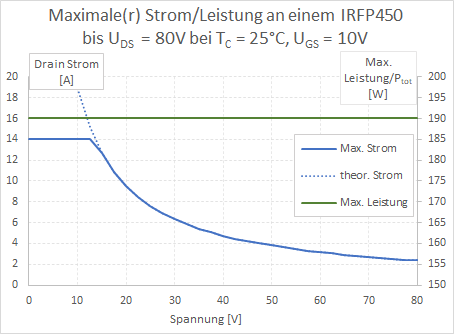
\includegraphics[width=0.5\textwidth]{Bilder/Irfp450_Strom_Spannung.png}
	\renewcommand*\figurename{Diagramm}
	\caption{Maximaler Strom in Abhängigkeit der Spannung unter Berücksichtigung von $P_{tot}$ an einem 
		IRFP450 \cite{IRFP450}}
	\label{dia:IRFP450_S_S_L}
\end{figure}
 
Im Diagramm \ref{dia:IRFP450_S_S_L} ist der Zusammenhang von maximalem Strom gegenüber der Spannung aufgezeigt. 
Der therotische Strom ist dabei über $P_{tot}$ berechnet.
Ein MOSFET-Halbleiter besitzt einen maximalen Drain-Strom, der ebenfalls beachtet werden muss.
Bei dem IRFP450 sind dies 14 Ampere\footnote{$T_{C} = $ 25°C und $U_{GS} = \SI{10}{\volt}$}.
Es ergibt sich die blaue Kurve (Max. Strom). $U_{DS,Q1}$ und $I_{D,Q1}$ darf jeden Wert unterhalb dieser Kurve annehmen. 
Oberhalb würde 
$P_{tot}$ überschritten werden. Gegen diesen Fehlerfall ist die Schaltung nicht gesichert.

\subsection{Fehlerrechnung}

Zu einer Schaltung sind deren Fehler stets anzugeben.
So werden folgend die Fehler und Beispielwerte aufgezeigt.
Die Schaltung der Widerstände $R4$ bis $R2$ werden hier nicht betrachtet, da die Referenzeinstellung über einem \grqq normalen\grqq{} 
Potentiometer eine reine Abschätzung ist und nach einer Anzeige eingestellt werden soll.
Für diese Anzeige sind die Schaltung \ref{sch:OP_Verstärkung}.1/.2 zuständig und werden folgend auf 
ihre Fehler untersucht.
Elektromagnetische Störungen werden ebenfalls nicht betrachtet da diese wie nach Abschnitt \ref{sec:EMV} 
stark minimiert werden können/sollten.\\

Der nicht-invertierende Verstärker macht hier den Anfang.
Neben den weit bekannten und oft schnell ersichtlichen Widerstandstoleranzen, sind die Operationsverstärkereingänge mit 
Eingangsströmen belastet. Diese können hinein oder heraus fließen und werden \textit{Input Bias Current} ($I_{B}$) genannt.
Somit kann eine Spannung am Ausgang der nicht-invertierenden Schaltung \ref{sch:OP_Verstärkung}.1 anliegen, 
ohne das durch $R1$ Strom fließt.  

\begin{equation}
	\Delta U_{R1,IB,ninv} = \biggl(1 + \frac{R11}{R10}\biggr) \cdot R10 \cdot I_{B}
\end{equation}

Neben diesem Fehler gibt es noch die Offset-Spannung. Diese beschreibt die mögliche Spannungsdifferenz 
zwischen den beiden Eingängen (+,-) und wird bei Verstärkung um diese verstärkt. 
Für die nicht-invertierende Schaltung gilt $V_{ges} = V_{U4}$.

\begin{equation}
	\label{eq:Delta_UOffset}
	\Delta U_{Offset} = U_{Offset} \cdot V_{ges}
\end{equation}

Nach der gauß´schen Fehlerfortpflanzung wird die Ausgangsgleichung partiell nach allen Fehlern abgeleitet und addiert.
Nach einsetzen der Formel \ref{eq:V*U_R1} (Ausgangsspannung des nicht-invertierenden Verstärkers) 
ergibt sich die Formel \ref{eq:ninv_Delta_V*U_R1} als Fehler der Verstärkerschaltung. 
Die zusätzlichen Offset- und Eingangsstrom-Fehler des Operationsverstärkers werden addiert. 

\begin{equation}
	\label{eq:V*U_R1}
	U_{R1,ninv} = \biggl(1 + \frac{R11}{R10}\biggr) \cdot R1 \cdot I_{L,max}
\end{equation}

\begin{multline}
	\label{eq:ninv_Delta_V*U_R1}
	\begin{split}
		\Delta U_{R1,ninv,max} 
						=&  \biggl( \biggl| \frac{\delta U_{R1,ninv}}{\delta R11} \biggr| \cdot \Delta R11 \biggr) \\ &+
							\biggl( \biggl| \frac{\delta U_{R1,ninv}}{\delta R10} \biggr| \cdot \Delta R10 \biggr) \\ &+ 
						 	\biggl( \biggl| \frac{\delta U_{R1,ninv}}{\delta R1}  \biggr| \cdot \Delta R1_{max} \biggr) \\ &+
							\Delta U_{R1,IB,ninv} + \Delta U_{Offset}\\
						=&  
							\biggl( \frac{R11}{R10^2} \cdot U_{R1,max} \cdot \Delta R10 \biggr) \\ &+ 
							\biggl( \frac{1}{R10} \cdot U_{R1,max} \cdot \Delta R11 \biggr) \\ &+
							\biggl( \biggl( 1 +\frac{R11}{R10}\biggr)\cdot I_{L,max} \cdot \Delta R1_{max} \biggr) \\ &+
							\Delta U_{R1,IB,ninv} + \Delta U_{Offset}\\
	\end{split}
\end{multline}


Die Toleranz ist von der OP Schaltung abhängig. Für den invertierenden Verstärker (Schaltung \ref{sch:OP_Verstärkung}.2) 
ergibt sich, ebenfalls nach der gauß´schen Fehlerfortpflanzung und Addition der Operationsverstärkerfehler, vereinfacht:

\begin{multline}
	\label{eq:inv_Delta_V*U_R1}
	\begin{split}
		\Delta U_{R1,inv,max} 
						=&  \biggl( \biggl(V_{U3} \cdot \frac{R7}{R6^2} \biggr) \cdot U_{R1,max} \cdot \Delta R6 \biggr) \\ &+
							\biggl( \biggl(V_{U3} \cdot \frac{1}{R6} \biggr) \cdot U_{R1,max} \cdot \Delta R7 \biggr) \\ &+ 
							\biggl( \biggl(V_{U2} \cdot \frac{R9}{R8^2} \biggr) \cdot U_{R1,max} \cdot \Delta R8 \biggr) \\ &+
							\biggl( \biggl(V_{U2} \cdot \frac{1}{R8} \biggr) \cdot U_{R1,max} \cdot \Delta R9 \biggr) \\ &+
							\biggl(V_{ges} \cdot I_{L,max} \cdot \Delta R1_{max} \biggr) \\ &+									% Fertig
							2 \cdot \Delta U_{R1,IB,inv} + 																		% Fertig
							2 \cdot \Delta U_{Offset}\\
	\end{split}
\end{multline}


In der Formel (\ref{eq:inv_Delta_V*U_R1}) darf es $2 \cdot \Delta U_{R1,IB,inv}$ heißen wenn $R6 = R8$.
Wenn nicht, wird $\Delta U_{R1,IB,inv}$ nach Formel \ref{eq:inv_Delta_IB} berechnet und darf in Formel \ref{eq:inv_Delta_V*U_R1} 
nicht mit zwei multipliziert werden.

\begin{equation}
	\label{eq:inv_Delta_IB}
	\Delta U_{R1,IB,inv} = (V_{ges} \cdot R6 \cdot I_{B}) + (V_{ges} \cdot R8 \cdot I_{B})
\end{equation}

Um den Fehler im gesamten Spannungsbereich $U_{R1}$ anzugeben zu können, müssen diese einzeln in 
lineare und absolute Fehler eingeteilt werden. 
Die Fehler $\Delta U_{Offset}$ und $\Delta U_{R1,IB}$ sind absolut und können bei einem Strom 
$I_{L} = \SI{0}{\ampere}$ auftreten.
Die restlichen sind lineare Fehler und von der aktuellen Spannung $U_{R1}$ abhängig. 
Die Formel \ref{eq:+-U_R1} gibt die Spannung plus minus den Fehler zu jener an.

\begin{equation}
	\label{eq:+-U_R1}
	\begin{split}
		U_{R1,(n)inv} \pm \bigg(&\sum \Delta U_{R1,absolut} \\
		&+ \frac{U_{R1,(n)inv}}{U_{R1,(n)inv,max}} \Big(\sum \Delta U_{R1,linear} \Big) \bigg)
	\end{split}
\end{equation}


\subsection{Beispiel für Fehler}

Als Beispiel sind hier die Fehler für beide Schaltungen (nach Tabelle \ref{tab:Werte_Fehler_Beispiel}, 
Seite \pageref{tab:Werte_Fehler_Beispiel} und \ref{tab:Fehler_Beispiel}) 
berechnet. Als Operationsverstärker wurde der LTC2057 \cite{LTC2057} angenommen. 
Das Beispiel aus \ref{sec:Bsp} ist Grundlage für dies ($I_{L,max} = \SI{7}{\ampere}$ usw.). 
Die maximale Temperatur für $R1$ wurde mit \SI{+60}{\degreeCelsius} empirisch festgelegt.

\begin{table}[!h]
	\centering
	\caption{Resultierende Fehler}
	\label{tab:Fehler_Beispiel}
	\normalsize
	\begin{tabular}{l|l|l|c}
		Fehlertyp & linear/ & Term &  Resultierender  \\
				  & absolut && Fehler\\
		\hline
	 	Allgemeine 		& linear 	& $\Delta R1$  				& 21,3 mV \\
						& absolut	& $\Delta U_{Offset}$		& 0,018 mV \\
		\hline
		N. Invertierend & linear 	& $\Delta R10$ 				& 21 mV \\
						& linear 	& $\Delta R11$ 				& 21 mV\\
						& absolut	& $\Delta U_{R1,IB,ninv}$	& 0,03 mV \\
		\hline
		Invertierend 	& linear 	& $\Delta R6$ 				& 28 mV\\
						& linear 	& $\Delta R7$ 				& 28 mV \\
						& linear	& $\Delta R8$ 				& 112 mV\\
						& linear	& $\Delta R9$ 				& 7 mV \\
						& absolut	& $\Delta U_{R1,IB,inv}$	& 0,01 mV \\
		
	\end{tabular}
\end{table}

Die Werte werden in Formel \ref{eq:+-U_R1} wie folgt eingetragen.
\begin{equation}
		U_{R1,ninv} \pm \bigg(0,048 mV
		+ \frac{U_{R1,ninv} \cdot 63,3mV}{2,8V}  \bigg)
\end{equation}

\begin{equation}
	U_{R1,inv} \pm \bigg(0,038 mV
	+ \frac{U_{R1,ninv} \cdot 196,3mV}{2,8V}  \bigg)
\end{equation}

An den Ausgängen der Schaltungen ergeben sich die maximalen Spannungen $U_{R1,ninv,max} = $ 2,8 V $\pm$ 0,063 V und 
$U_{R1,inv,max} = $ 2,8 V $\pm$ 0,196 V. 

In Tabelle \ref{tab:Fehler_Beispiel} ist zu erkennen, dass die Fehler des Input Bias Current und der Offset Spannung sehr klein sind.
	
	\section{Mögliche Erweiterung}

Wenn für $U1$ ein Operationsverstärker mit Disable/Shutdown Pin verwendet wird, können mehrere Lasten mit 
verschiedenen $I_{L,max}$ parallel geschaltet werden. 
Es wäre nur eine Referenz nötig. 
So kann in einem Gerät eine breitbandige genaue 
(nach Abschnitt \ref{sec:Grenzen}) Stromsenke realisiert werden. 
Beispiel: $I_{L1,max} = \SI{100}{m\ampere}, I_{L2,max} = \SI{1}{\ampere}, I_{L3,max} = \SI{10}{\ampere}$.\\

Wenn nun mehrere Spannungsreferenzen zur Verfügung stehen, können nach dem Kirchhoffschen-Knotenpunktsatz auch \grqq Mischgrößen\grqq{} 
gebaut werden.
Beispiel: $I_{L,max} = \SI{1,2}{\ampere}$ ($\SI{1}{\ampere}$ und $\SI{200}{m\ampere}$)\\


Wie schon im Artikel angedeutet, wäre eine Erweiterungsmöglichkeit, andere Fehlerarten der Schaltung 
mit einem Mikrocontroller zu verhindern.
Informationswerte, wie aktueller Stromfluss und Spannung, können an einem Display angezeigt werden.
So könnte beispielsweise eine Temperaturüberwachung am Kühlkörper realisiert werden.
Bei überschreiten der Grenztemperatur kann der Shutdown des OP`s genutzt werden, um den MOSFET hochohmig zu schalten.
Mit einem weiteren ADC Eingang, über einen Spannungsteiler gemessen, kann $P_{Q1} = (U_{L} - R1 \cdot I_{L}) \cdot I_{L}$ bzw. 
$P_{L} = U_{L} \cdot I_{L}$ berechnet werden. 
Ein akustisches oder visuelles Signal kann so vor den bevorstehenden Überschreitungen von 
$U_{DS,Q1}$, $I_{D,Q1}$ und/oder $P_{tot,Q1}$, den Nutzer warnen.\\

Wer ein passendes Analogmessinstrument hat, kann die Anzeige auch im Retrostil bauen.
	
	\begin{thebibliography}{1}		
		\bibitem{LL_MOSFET}	
		Falk (Username mikrocontroller.net), \emph{MOSFET-Übersicht}\hskip 1em plus
		0.5em minus 0.4em \relax https://www.mikrocontroller.net/articles/MOSFET-Übersicht, 07.02.2021, Letzter Aufruf 23.04.2021
		
		\bibitem{IRFP450}	
		Vishay Siliconix, \emph{Datasheet Power MOSFET, IRFP450, SiHFP450}\hskip 1em plus
		0.5em minus 0.4em \relax https://www.vishay.com/docs/91233/91233.pdf, 16.06.2008, Letzter Aufruf 23.04.2021
		
		\bibitem{IRFP250}
		Vishay Siliconix, \emph{Datasheet Power MOSFET, IRFP240, SiHFP240}\hskip 1em plus
		0.5em minus 0.4em \relax https://www.vishay.com/docs/91210/91210.pdf, 21.03.2011, Letzter Aufruf 19.05.2021
		
		\bibitem{LTC2057}
		Analog Devices, \emph{LTC2057: High Voltage, Low Noise Zero-Drift Operational Amplifier Data Sheet} \hskip 1em plus
		0.5em minus 0.4em \relax https://www.analog.com/media/en/technical-documentation/data-sheets/2057f.pdf, Letzter Aufruf 16.04.2021
		
		\bibitem{E-Reihen}
		Manfred Hein, \emph{DIE IEC- WERTETABELLEN} \hskip 1em plus
		0.5em minus 0.4em \relax http://www.heinffm.de/0199d9924f0e9e80e/0199d9924f0eb3f3b/0199d992cf1014103/, Letzter Aufruf 05.05.2021
		
		\bibitem{TCR_rechnen}
		Prof. Dr. Wolfgang Matthes, \emph{Widerstände} \hskip 1em plus
		0.5em minus 0.4em \relax http://www.controllersandpcs.de/lehrarchiv/pdfs/elektronik/pass01\_01x.pdf, Letzter Aufruf 11.05.2021
		
	\end{thebibliography}
\end{document}